\documentclass{rapportENSIAS}
\usepackage[utf8]{inputenc}
\usepackage{float}


\usepackage{graphicx}
\usepackage{listings}
\usepackage{xcolor}
\usepackage{float}

\lstset{
    basicstyle=\ttfamily\small,
    backgroundcolor=\color{gray!40},
    frame=single,
    breaklines=true
}

\usepackage{lipsum}
\usepackage{minted}
\usepackage{caption}
\usepackage{float}
\usepackage{color}
\usepackage{amssymb}
\usepackage{pifont} 

\usepackage{xcolor}
\usepackage{graphicx}
\usepackage{amsmath}

% \usepackage[utf8x]{inputenc}
\usepackage[T1]{fontenc}
\usepackage[french]{babel}
\usepackage{graphicx}
\usepackage{geometry}
\usepackage{xcolor}
\usepackage{enumitem}
\usepackage{fancyhdr}
\usepackage{tikz}
\usepackage{tcolorbox}




% Configuration personnalisée pour le code assembleur

\definecolor{bg}{rgb}{0.95,0.95,0.95} % Adjust the RGB values as needed
\title{Rapport Enset - Template} %Titre du fichier



\definecolor{winblue}{RGB}{0,120,215}
\definecolor{lightgray}{RGB}{240,240,240}

\definecolor{javared}{rgb}{0.6,0,0}
\definecolor{javagreen}{rgb}{0.25,0.5,0.35}
\definecolor{javapurple}{rgb}{0.5,0,0.35}
\definecolor{javadocblue}{rgb}{0.25,0.35,0.75}
\definecolor{codebackground}{rgb}{0.95,0.95,0.92}

\lstset{
    language=Java,
    basicstyle=\ttfamily\small,
    keywordstyle=\color{javapurple}\bfseries,
    stringstyle=\color{javared},
    commentstyle=\color{javagreen},
    morecomment=[s][\color{javadocblue}]{/**}{*/},
    numbers=left,
    numberstyle=\tiny\color{black},
    stepnumber=1,
    numbersep=10pt,
    tabsize=4,
    showspaces=false,
    showstringspaces=false,
    backgroundcolor=\color{codebackground},
    frame=single,
    captionpos=b,
    breaklines=true,
    breakatwhitespace=false,
    escapeinside={(*@}{@*)}
}


\lstset{
    basicstyle=\ttfamily\small,
    keywordstyle=\color{winblue},
    breaklines=true,
}

% ====== MANUAL FRENCH CHARACTER HANDLING ======
\newcommand{\eacute}{\'{e}}      % é
\newcommand{\egrave}{\`{e}}      % è
\newcommand{\ecirc}{\^{e}}       % ê
\newcommand{\ccedil}{\c{c}}      % ç
\newcommand{\agrave}{\`{a}}      % à
\newcommand{\acirc}{\^{a}}       % â
\newcommand{\icirc}{\^{i}}       % î
\newcommand{\ocirc}{\^{o}}       % ô
\newcommand{\ucirc}{\^{u}}       % û
\newcommand{\Eacute}{\'{E}}      % É
\newcommand{\Ccedil}{\c{C}}      % Ç

\begin{document}

%----------- Informations du rapport ---------

\titre{Application de Gestion de Livraison de Colis} %Titre du fichier .pdf
%\UE{UE PRO} %Nom de la UE
\sujet{Module : Conception et programmation POO}%Nom du sujet

\enseignant{M. Abdelmajid \textsc{BOUSSELHAM}} %Nom de l'enseignant

\eleves{Yasser \textsc{Namez} } %Nom des élèves

%----------- Initialisation -------------------
        
\fairemarges %Afficher les marges
\fairepagedegarde %Créer la page de garde
\tabledematieres %Créer la table de matières


%------------ Corps du rapport ----------------

\section{Introduction}

Ce rapport pr\'{e}sente une application de gestion de livraison de colis d\'{e}velopp\'{e}e en Java avec JavaFX. L'application permet de g\'{e}rer les colis, les livreurs et les op\'{e}rations de livraison dans un syst\`{e}me centralis\'{e}.

\subsection{Objectif du Projet}

L'objectif principal est de cr\'{e}er une application desktop permettant de :
\begin{itemize}
    \item G\'{e}rer les colis (ajout, modification, suppression)
    \item G\'{e}rer les livreurs (ajout, modification, suppression)
    \item Assigner des colis aux livreurs
    \item Suivre le statut des livraisons
    \item Exporter les donn\'{e}es de livraison au format CSV
\end{itemize}

\subsection{Technologies Utilis\'{e}es}

\begin{itemize}
    \item \textbf{Java} : Langage de programmation principal
    \item \textbf{JavaFX} : Framework pour l'interface utilisateur
    \item \textbf{FXML} : Format XML pour la d\'{e}finition des interfaces
    \item \textbf{JDBC} : Acc\`{e}s aux donn\'{e}es
    \item \textbf{CSS} : Stylisation de l'interface
    \item \textbf{Maven} : Gestionnaire de d\'{e}pendances
\end{itemize}

\section{Architecture du Syst\`{e}me}

\subsection{Diagramme de Cas d'Utilisation}

\begin{figure}[H]
    \centering
    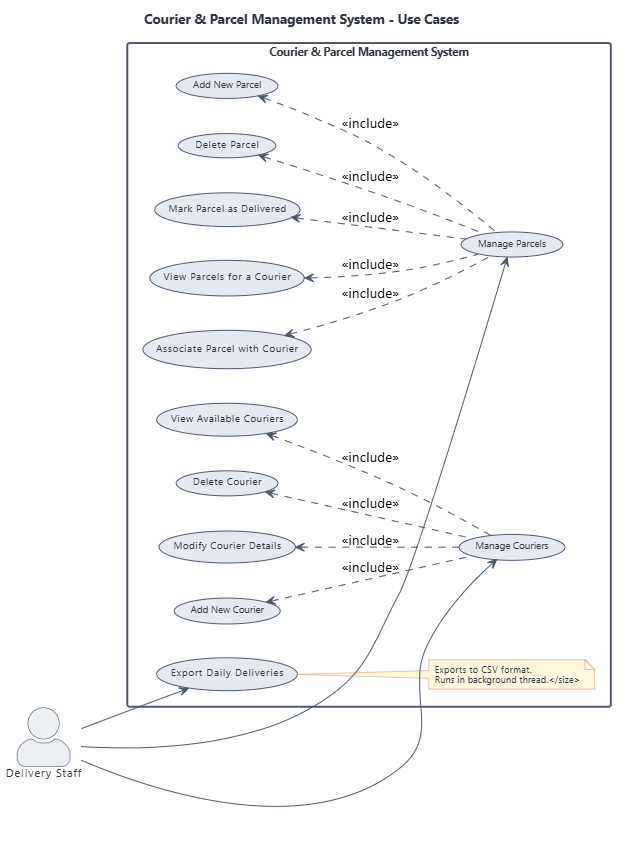
\includegraphics[width=0.8\textwidth]{UseCase Diagram.png}
    \caption{Diagramme de cas d'utilisation}
    \label{fig:usecase}
\end{figure}

Le diagramme de cas d'utilisation illustre les principales fonctionnalit\'{e}s de l'application et les interactions entre les utilisateurs et le syst\`{e}me.

\subsection{Diagramme de Classes}

\begin{figure}[H]
    \centering
    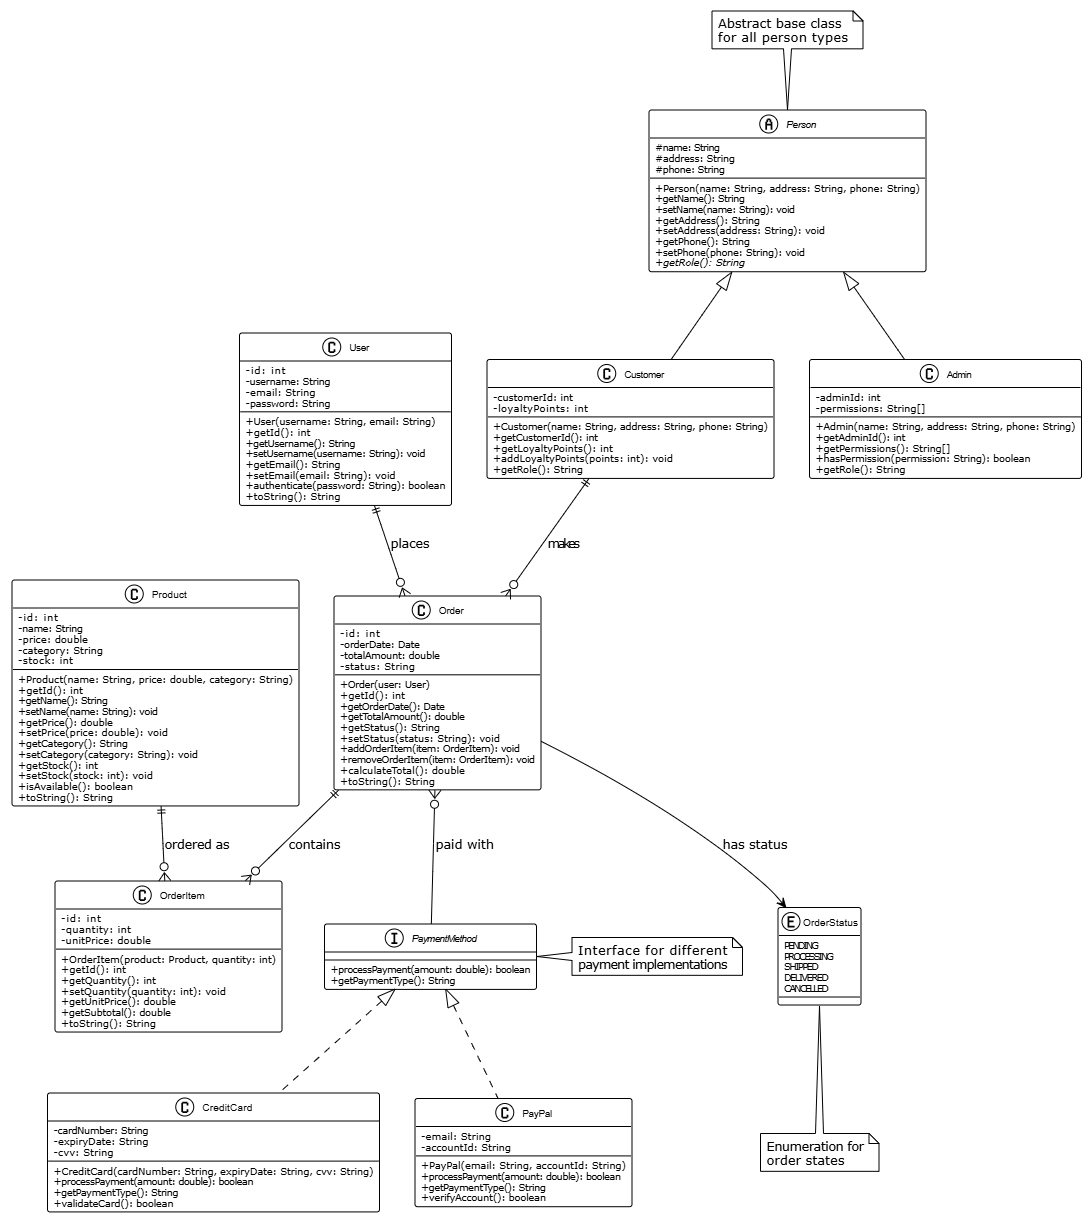
\includegraphics[width=\textwidth]{class diagram.png}
    \caption{Diagramme de classes}
    \label{fig:classdiagram}
\end{figure}

Le diagramme de classes montre la structure orient\'{e}e objet de l'application avec les principales entit\'{e}s, leurs attributs et relations.

\subsection{Mod\`{e}le Logique de Donn\'{e}es (MLD)}

\begin{figure}[H]
    \centering
    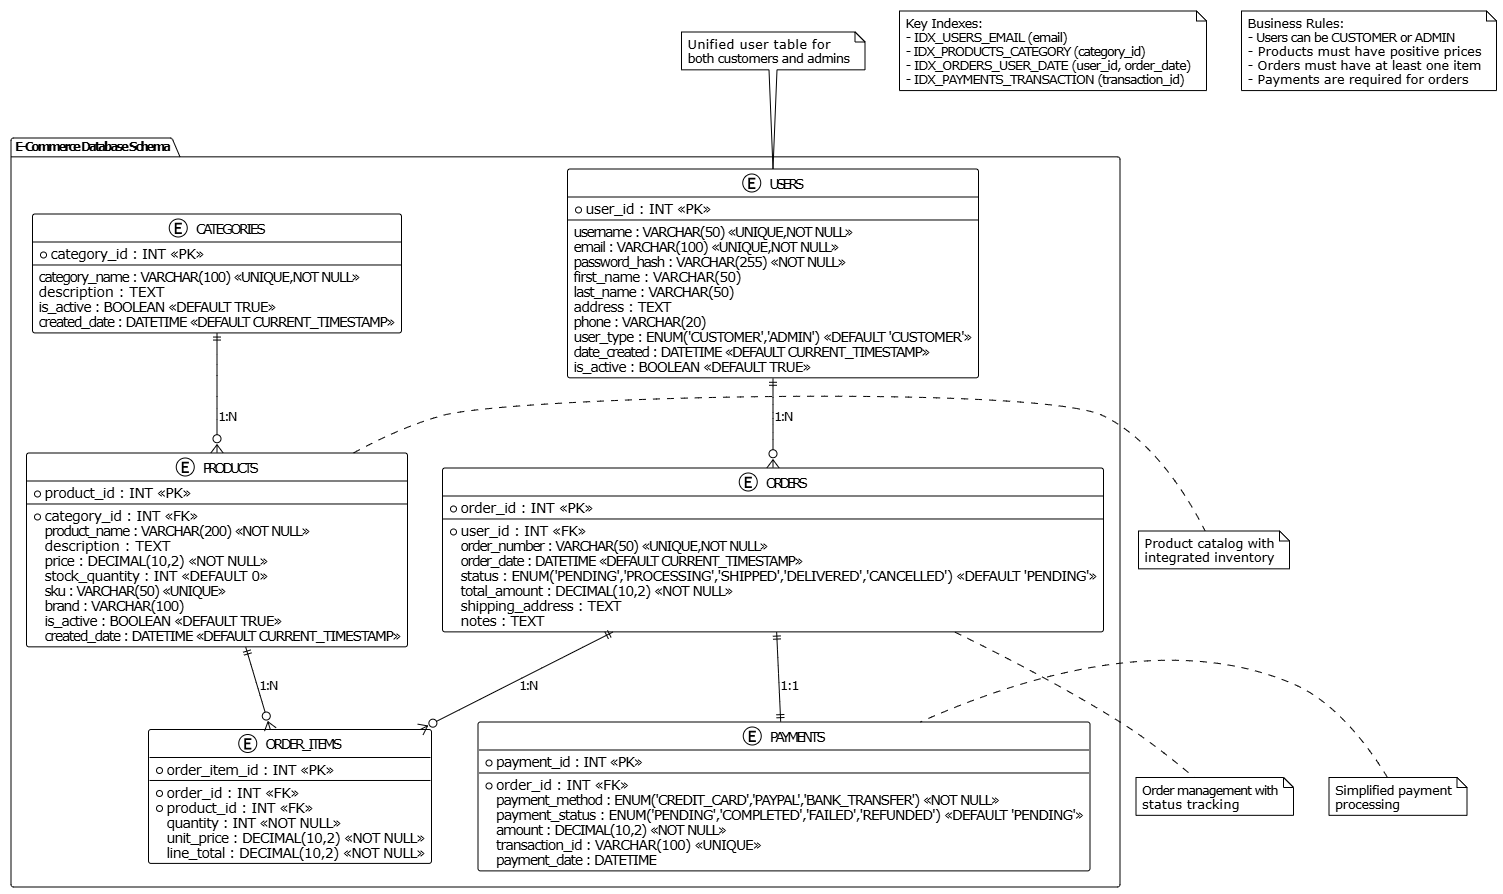
\includegraphics[width=0.9\textwidth]{MLD.png}
    \caption{Mod\`{e}le Logique de Donn\'{e}es}
    \label{fig:mld}
\end{figure}

Le MLD pr\'{e}sente la structure de la base de donn\'{e}es avec les tables et leurs relations.

\section{Architecture du Code}

L'application suit une architecture en couches (layered architecture) organis\'{e}e comme suit :

\subsection{Package Structure}

\begin{lstlisting}[language=Java, caption=Structure des packages]
com.example.deliveryapp/
├── app/               // Point d'entrée de l'application
├── controller/        // Contrôleurs JavaFX (MVC)
├── dao/              // Data Access Objects
├── entities/         // Entités métier
├── service/          // Logique métier
└── util/             // Utilitaires
\end{lstlisting}

\subsection{Couche Entit\'{e}s (Entities)}

Les entit\'{e}s repr\'{e}sentent les objets m\'{e}tier principaux :

\subsubsection{Classe Colis}

\begin{lstlisting}[language=Java, caption=Entit\'{e} Colis]
public class Colis {
    private int id;
    private String destinataire;
    private String adresse;
    private LocalDate dateEnvoi;
    private boolean livre;
    private LocalDate dateLivraison;
    private Integer livreurId;
    private Livreur livreur;
    
    // Constructeurs
    public Colis() {}
    
    public Colis(String destinataire, String adresse, LocalDate dateEnvoi) {
        this.destinataire = destinataire;
        this.adresse = adresse;
        this.dateEnvoi = dateEnvoi;
        this.livre = false;
    }
    
    // Getters et Setters...
    
    public String getStatutText() {
        return livre ? "Livré" : "Non livré";
    }
    
    public String getLivreurName() {
        return livreur != null ? livreur.getFullName() : "";
    }
}
\end{lstlisting}

\subsubsection{Classe Livreur}

\begin{lstlisting}[language=Java, caption=Entit\'{e} Livreur]
public class Livreur {
    private int id;
    private String nom;
    private String prenom;
    private String telephone;
    
    // Constructeurs
    public Livreur() {}
    
    public Livreur(String nom, String prenom, String telephone) {
        this.nom = nom;
        this.prenom = prenom;
        this.telephone = telephone;
    }
    
    // Getters et Setters...
    
    @Override
    public String toString() {
        return prenom + " " + nom;
    }
    
    public String getFullName() {
        return prenom + " " + nom;
    }
}
\end{lstlisting}

\subsection{Couche DAO (Data Access Objects)}

La couche DAO g\`{e}re l'acc\`{e}s aux donn\'{e}es.

\subsubsection{Interface IColisDAO}

\begin{lstlisting}[language=Java, caption=Interface IColisDAO]
public interface IColisDAO {
    void addColis(Colis colis) throws Exception;
    void updateColis(Colis colis) throws Exception;
    void deleteColis(int id) throws Exception;
    Colis getColisById(int id) throws Exception;
    List<Colis> getAllColis() throws Exception;
    List<Colis> getColisByLivreurId(int livreurId) throws Exception;
    List<Colis> getColisDeliveredOnDate(LocalDate date) throws Exception;
}
\end{lstlisting}

\subsubsection{Impl\'{e}mentation ColisDAOImpl Compl\`{e}te}

\begin{lstlisting}[language=Java, caption=Impl\'{e}mentation ColisDAOImpl compl\`{e}te]
package com.example.deliveryapp.dao;

import com.example.deliveryapp.entities.Colis;
import com.example.deliveryapp.entities.Livreur;
import com.example.deliveryapp.util.DatabaseManager;

import java.sql.*;
import java.time.LocalDate;
import java.util.ArrayList;
import java.util.List;

/**
 * Implementation of IColisDAO using JDBC
 */
public class ColisDAOImpl implements IColisDAO {
    
    @Override
    public void addColis(Colis colis) throws Exception {
        String sql = "INSERT INTO colis (destinataire, adresse, dateEnvoi, livre, dateLivraison, livreur_id) VALUES (?, ?, ?, ?, ?, ?)";
        
        try (Connection conn = DatabaseManager.getConnection();
             PreparedStatement stmt = conn.prepareStatement(sql, Statement.RETURN_GENERATED_KEYS)) {
            
            stmt.setString(1, colis.getDestinataire());
            stmt.setString(2, colis.getAdresse());
            stmt.setDate(3, Date.valueOf(colis.getDateEnvoi()));
            stmt.setBoolean(4, colis.isLivre());
            stmt.setDate(5, colis.getDateLivraison() != null ? Date.valueOf(colis.getDateLivraison()) : null);
            stmt.setObject(6, colis.getLivreurId());
            
            int affectedRows = stmt.executeUpdate();
            if (affectedRows == 0) {
                throw new SQLException("Creating colis failed, no rows affected.");
            }
            
            try (ResultSet generatedKeys = stmt.getGeneratedKeys()) {
                if (generatedKeys.next()) {
                    colis.setId(generatedKeys.getInt(1));
                } else {
                    throw new SQLException("Creating colis failed, no ID obtained.");
                }
            }
        }
    }
    
    @Override
    public void updateColis(Colis colis) throws Exception {
        String sql = "UPDATE colis SET destinataire = ?, adresse = ?, dateEnvoi = ?, livre = ?, dateLivraison = ?, livreur_id = ? WHERE id = ?";
        
        try (Connection conn = DatabaseManager.getConnection();
             PreparedStatement stmt = conn.prepareStatement(sql)) {
            
            stmt.setString(1, colis.getDestinataire());
            stmt.setString(2, colis.getAdresse());
            stmt.setDate(3, Date.valueOf(colis.getDateEnvoi()));
            stmt.setBoolean(4, colis.isLivre());
            stmt.setDate(5, colis.getDateLivraison() != null ? Date.valueOf(colis.getDateLivraison()) : null);
            stmt.setObject(6, colis.getLivreurId());
            stmt.setInt(7, colis.getId());
            
            int affectedRows = stmt.executeUpdate();
            if (affectedRows == 0) {
                throw new SQLException("Updating colis failed, no rows affected.");
            }
        }
    }
    
    @Override
    public void deleteColis(int id) throws Exception {
        String sql = "DELETE FROM colis WHERE id = ?";
        
        try (Connection conn = DatabaseManager.getConnection();
             PreparedStatement stmt = conn.prepareStatement(sql)) {
            
            stmt.setInt(1, id);
            
            int affectedRows = stmt.executeUpdate();
            if (affectedRows == 0) {
                throw new SQLException("Deleting colis failed, no rows affected.");
            }
        }
    }
    
    @Override
    public Colis getColisById(int id) throws Exception {
        String sql = "SELECT c.*, l.nom as livreur_nom, l.prenom as livreur_prenom, l.telephone as livreur_telephone " +
                    "FROM colis c LEFT JOIN livreurs l ON c.livreur_id = l.id WHERE c.id = ?";
        
        try (Connection conn = DatabaseManager.getConnection();
             PreparedStatement stmt = conn.prepareStatement(sql)) {
            
            stmt.setInt(1, id);
            
            try (ResultSet rs = stmt.executeQuery()) {
                if (rs.next()) {
                    return mapResultSetToColis(rs);
                }
            }
        }
        return null;
    }
    
    @Override
    public List<Colis> getAllColis() throws Exception {
        String sql = "SELECT c.*, l.nom as livreur_nom, l.prenom as livreur_prenom, l.telephone as livreur_telephone " +
                    "FROM colis c LEFT JOIN livreurs l ON c.livreur_id = l.id ORDER BY c.dateEnvoi DESC";
        List<Colis> colisList = new ArrayList<>();
        
        try (Connection conn = DatabaseManager.getConnection();
             PreparedStatement stmt = conn.prepareStatement(sql);
             ResultSet rs = stmt.executeQuery()) {
            
            while (rs.next()) {
                colisList.add(mapResultSetToColis(rs));
            }
        }
        
        return colisList;
    }
    
    @Override
    public List<Colis> getColisByLivreurId(int livreurId) throws Exception {
        String sql = "SELECT c.*, l.nom as livreur_nom, l.prenom as livreur_prenom, l.telephone as livreur_telephone " +
                    "FROM colis c LEFT JOIN livreurs l ON c.livreur_id = l.id WHERE c.livreur_id = ? ORDER BY c.dateEnvoi DESC";
        List<Colis> colisList = new ArrayList<>();
        
        try (Connection conn = DatabaseManager.getConnection();
             PreparedStatement stmt = conn.prepareStatement(sql)) {
            
            stmt.setInt(1, livreurId);
            
            try (ResultSet rs = stmt.executeQuery()) {
                while (rs.next()) {
                    colisList.add(mapResultSetToColis(rs));
                }
            }
        }
        
        return colisList;
    }
    
    @Override
    public List<Colis> getColisDeliveredOnDate(LocalDate date) throws Exception {
        String sql = "SELECT c.*, l.nom as livreur_nom, l.prenom as livreur_prenom, l.telephone as livreur_telephone " +
                    "FROM colis c LEFT JOIN livreurs l ON c.livreur_id = l.id WHERE c.dateLivraison = ? ORDER BY c.id";
        List<Colis> colisList = new ArrayList<>();
        
        try (Connection conn = DatabaseManager.getConnection();
             PreparedStatement stmt = conn.prepareStatement(sql)) {
            
            stmt.setDate(1, Date.valueOf(date));
            
            try (ResultSet rs = stmt.executeQuery()) {
                while (rs.next()) {
                    colisList.add(mapResultSetToColis(rs));
                }
            }
        }
        
        return colisList;
    }
    
    /**
     * Helper method to map ResultSet to Colis object
     */
    private Colis mapResultSetToColis(ResultSet rs) throws SQLException {
        Colis colis = new Colis();
        colis.setId(rs.getInt("id"));
        colis.setDestinataire(rs.getString("destinataire"));
        colis.setAdresse(rs.getString("adresse"));
        
        Date dateEnvoi = rs.getDate("dateEnvoi");
        if (dateEnvoi != null) {
            colis.setDateEnvoi(dateEnvoi.toLocalDate());
        }
        
        colis.setLivre(rs.getBoolean("livre"));
        
        Date dateLivraison = rs.getDate("dateLivraison");
        if (dateLivraison != null) {
            colis.setDateLivraison(dateLivraison.toLocalDate());
        }
        
        Object livreurIdObj = rs.getObject("livreur_id");
        if (livreurIdObj != null) {
            colis.setLivreurId((Integer) livreurIdObj);
            
            // Create Livreur object if data is available
            String livreurNom = rs.getString("livreur_nom");
            if (livreurNom != null) {
                Livreur livreur = new Livreur(
                    colis.getLivreurId(),
                    livreurNom,
                    rs.getString("livreur_prenom"),
                    rs.getString("livreur_telephone")
                );
                colis.setLivreur(livreur);
            }
        }
        
        return colis;
    }
}
\end{lstlisting}

\subsection{Couche Service}

La couche service contient la logique m\'{e}tier.

\subsubsection{Interface IColisService}

\begin{lstlisting}[language=Java, caption=Interface IColisService]
public interface IColisService {
    void addColis(Colis colis) throws Exception;
    void updateColis(Colis colis) throws Exception;
    void deleteColis(int id) throws Exception;
    Colis getColisById(int id);
    List<Colis> getAllColis();
    void assignColisToLivreur(int colisId, int livreurId) throws Exception;
    List<Colis> getColisByLivreur(int livreurId);
    void markColisAsDelivered(int colisId) throws Exception;
    List<Colis> getColisDeliveredToday();
    String exportDeliveredTodayToCSV() throws Exception;
}
\end{lstlisting}

\subsubsection{Impl\'{e}mentation ColisServiceImpl Compl\`{e}te}

\begin{lstlisting}[language=Java, caption=Service Colis avec validation compl\`{e}te]
package com.example.deliveryapp.service;

import com.example.deliveryapp.dao.IColisDAO;
import com.example.deliveryapp.dao.ColisDAOImpl;
import com.example.deliveryapp.entities.Colis;
import com.example.deliveryapp.util.CSVExporter;

import java.time.LocalDate;
import java.util.ArrayList;
import java.util.List;

/**
 * Implementation of IColisService
 */
public class ColisServiceImpl implements IColisService {
    private final IColisDAO colisDAO;
    private final CSVExporter csvExporter;
    
    public ColisServiceImpl() {
        this.colisDAO = new ColisDAOImpl();
        this.csvExporter = new CSVExporter();
    }
    
    @Override
    public void addColis(Colis colis) throws Exception {
        validateColis(colis);
        colisDAO.addColis(colis);
    }
    
    @Override
    public void updateColis(Colis colis) throws Exception {
        validateColis(colis);
        if (colis.getId() <= 0) {
            throw new Exception("ID du colis invalide pour la mise à jour");
        }
        colisDAO.updateColis(colis);
    }
    
    @Override
    public void deleteColis(int id) throws Exception {
        if (id <= 0) {
            throw new Exception("ID du colis invalide");
        }
        colisDAO.deleteColis(id);
    }
    
    @Override
    public Colis getColisById(int id) {
        try {
            return colisDAO.getColisById(id);
        } catch (Exception e) {
            System.err.println("Error getting colis by ID: " + e.getMessage());
            return null;
        }
    }
    
    @Override
    public List<Colis> getAllColis() {
        try {
            return colisDAO.getAllColis();
        } catch (Exception e) {
            System.err.println("Error getting all colis: " + e.getMessage());
            return new ArrayList<>();
        }
    }
    
    @Override
    public void assignColisToLivreur(int colisId, int livreurId) throws Exception {
        if (colisId <= 0) {
            throw new Exception("ID du colis invalide");
        }
        if (livreurId <= 0) {
            throw new Exception("ID du livreur invalide");
        }
        
        Colis colis = colisDAO.getColisById(colisId);
        if (colis == null) {
            throw new Exception("Colis non trouvé");
        }
        
        colis.setLivreurId(livreurId);
        colisDAO.updateColis(colis);
    }
    
    @Override
    public List<Colis> getColisByLivreur(int livreurId) {
        try {
            return colisDAO.getColisByLivreurId(livreurId);
        } catch (Exception e) {
            System.err.println("Error getting colis by livreur: " + e.getMessage());
            return new ArrayList<>();
        }
    }
    
    @Override
    public void markColisAsDelivered(int colisId) throws Exception {
        if (colisId <= 0) {
            throw new Exception("ID du colis invalide");
        }
        
        Colis colis = colisDAO.getColisById(colisId);
        if (colis == null) {
            throw new Exception("Colis non trouvé");
        }
        
        if (colis.isLivre()) {
            throw new Exception("Ce colis est déjà marqué comme livré");
        }
        
        colis.setLivre(true);
        colis.setDateLivraison(LocalDate.now());
        colisDAO.updateColis(colis);
    }
    
    @Override
    public List<Colis> getColisDeliveredToday() {
        try {
            return colisDAO.getColisDeliveredOnDate(LocalDate.now());
        } catch (Exception e) {
            System.err.println("Error getting colis delivered today: " + e.getMessage());
            return new ArrayList<>();
        }
    }
    
    @Override
    public String exportDeliveredTodayToCSV() throws Exception {
        List<Colis> deliveredToday = getColisDeliveredToday();
        return csvExporter.exportColisToCSV(deliveredToday);
    }
    
    /**
     * Validate Colis data
     * @param colis The colis to validate
     * @throws Exception if validation fails
     */
    private void validateColis(Colis colis) throws Exception {
        if (colis == null) {
            throw new Exception("Les données du colis ne peuvent pas être nulles");
        }
        
        if (colis.getDestinataire() == null || colis.getDestinataire().trim().isEmpty()) {
            throw new Exception("Le destinataire du colis est obligatoire");
        }
        
        if (colis.getAdresse() == null || colis.getAdresse().trim().isEmpty()) {
            throw new Exception("L'adresse du colis est obligatoire");
        }
        
        if (colis.getDateEnvoi() == null) {
            throw new Exception("La date d'envoi du colis est obligatoire");
        }
        
        if (colis.getDateEnvoi().isAfter(LocalDate.now())) {
            throw new Exception("La date d'envoi ne peut pas être dans le futur");
        }
    }
}
\end{lstlisting}

\subsection{Couche Contr\^{o}leur}

Les contr\^{o}leurs g\`{e}rent l'interaction entre l'interface utilisateur et la logique m\'{e}tier.

\subsubsection{ColisController}

\begin{lstlisting}[language=Java, caption=Contr\^{o}leur Colis (extrait)]
public class ColisController implements Initializable {
    @FXML private TextField destinataireField;
    @FXML private TextArea adresseField;
    @FXML private DatePicker dateEnvoiPicker;
    @FXML private ComboBox<Livreur> livreurComboBox;
    @FXML private TableView<Colis> colisTable;
    
    private IColisService colisService;
    private ILivreurService livreurService;
    private ObservableList<Colis> colisList;
    private Colis selectedColis;
    
    @Override
    public void initialize(URL url, ResourceBundle resourceBundle) {
        colisService = new ColisServiceImpl();
        livreurService = new LivreurServiceImpl();
        
        setupTable();
        setupForm();
        loadData();
        setupEventHandlers();
    }
    
    @FXML
    private void handleAddColis() {
        if (!validateForm()) return;
        
        try {
            Colis newColis = createColisFromForm();
            colisService.addColis(newColis);
            
            AlertUtils.showSuccess("Succès", "Colis ajouté avec succès.");
            loadColis();
            clearForm();
            
        } catch (Exception e) {
            AlertUtils.showError("Erreur d'Ajout", 
                "Impossible d'ajouter le colis", e.getMessage());
        }
    }
    
    @FXML
    private void handleAssignToDriver() {
        if (selectedColis == null || selectedColis.isLivre()) return;
        
        Livreur selectedLivreur = livreurComboBox.getValue();
        if (selectedLivreur == null) {
            AlertUtils.showWarning("Sélection", "Aucun livreur sélectionné", 
                "Veuillez sélectionner un livreur.");
            return;
        }
        
        try {
            colisService.assignColisToLivreur(selectedColis.getId(), 
                selectedLivreur.getId());
            AlertUtils.showSuccess("Succès", 
                "Colis assigné avec succès au livreur " + 
                selectedLivreur.getFullName() + ".");
            loadColis();
        } catch (Exception e) {
            AlertUtils.showError("Erreur d'Assignation", 
                "Impossible d'assigner le colis", e.getMessage());
        }
    }
}
\end{lstlisting}

\section{Interfaces Utilisateur}

\subsection{Interface Principale}

\begin{figure}[H]
    \centering
    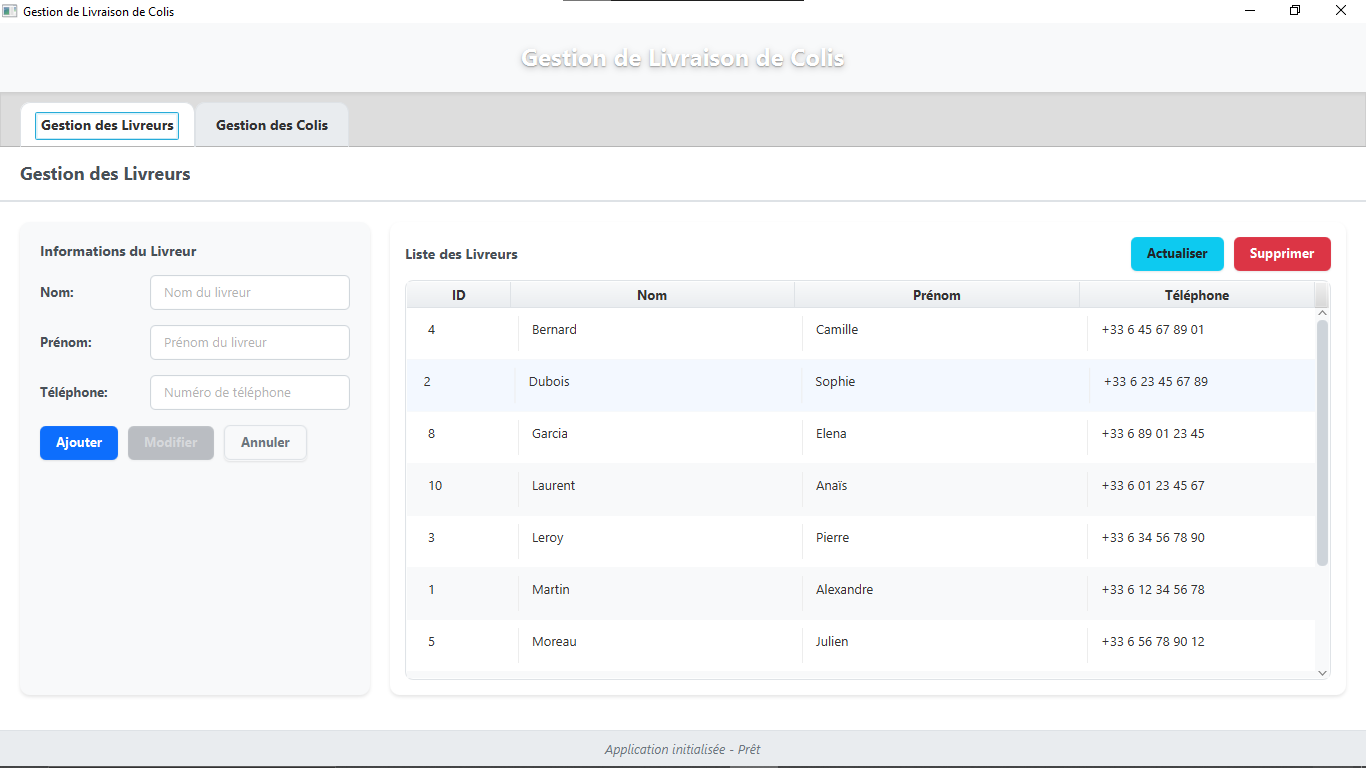
\includegraphics[width=\textwidth]{interface1.png}
    \caption{Interface principale - Gestion des colis}
    \label{fig:interface1}
\end{figure}

L'interface principale permet de :
\begin{itemize}
    \item Visualiser la liste de tous les colis
    \item Ajouter, modifier et supprimer des colis
    \item Assigner des colis aux livreurs
    \item Marquer les colis comme livr\'{e}s
    \item Exporter les livraisons du jour en CSV
\end{itemize}

\subsection{Interface de Gestion des Livreurs}

\begin{figure}[H]
    \centering
    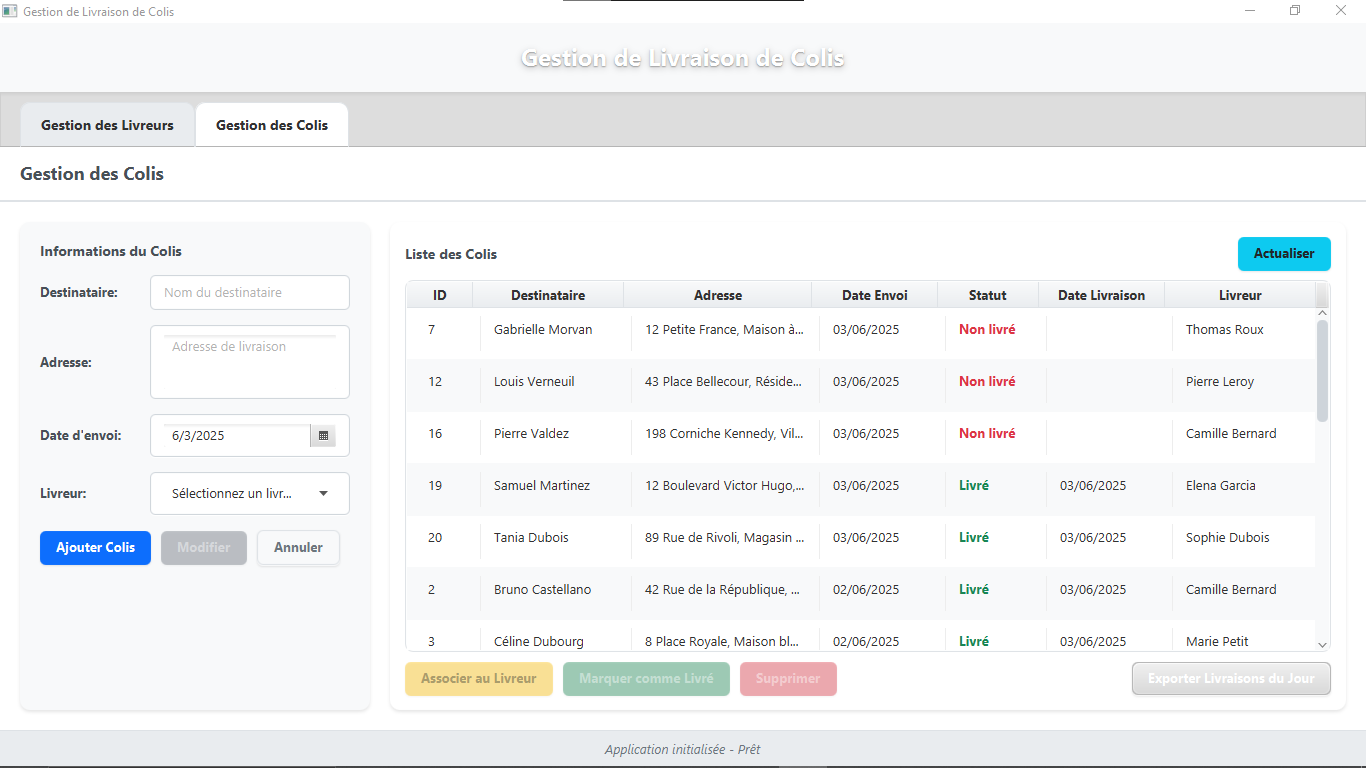
\includegraphics[width=\textwidth]{interface2.png}
    \caption{Interface de gestion des livreurs}
    \label{fig:interface2}
\end{figure}

Cette interface permet de :
\begin{itemize}
    \item Visualiser la liste des livreurs
    \item Ajouter de nouveaux livreurs
    \item Modifier les informations des livreurs existants
    \item Supprimer des livreurs
\end{itemize}

\section{Fonctionnalit\'{e}s Principales}

\subsection{Gestion des Colis}

\subsubsection{Ajout de Colis}
L'application permet d'ajouter de nouveaux colis avec validation des donn\'{e}es :

\begin{lstlisting}[language=Java, caption=Validation des colis]
private boolean validateForm() {
    if (destinataireField.getText().trim().isEmpty()) {
        AlertUtils.showWarning("Validation", "Champ requis", 
            "Le destinataire est obligatoire.");
        destinataireField.requestFocus();
        return false;
    }
    
    if (adresseField.getText().trim().isEmpty()) {
        AlertUtils.showWarning("Validation", "Champ requis", 
            "L'adresse est obligatoire.");
        adresseField.requestFocus();
        return false;
    }
    
    if (dateEnvoiPicker.getValue() == null) {
        AlertUtils.showWarning("Validation", "Champ requis", 
            "La date d'envoi est obligatoire.");
        dateEnvoiPicker.requestFocus();
        return false;
    }
    
    return true;
}
\end{lstlisting}

\subsubsection{Assignation aux Livreurs}
Les colis peuvent \^{e}tre assign\'{e}s aux livreurs disponibles :

\begin{lstlisting}[language=Java, caption=Assignation de colis]
@Override
public void assignColisToLivreur(int colisId, int livreurId) throws Exception {
    if (colisId <= 0) {
        throw new Exception("ID du colis invalide");
    }
    if (livreurId <= 0) {
        throw new Exception("ID du livreur invalide");
    }
    
    Colis colis = colisDAO.getColisById(colisId);
    if (colis == null) {
        throw new Exception("Colis non trouvé");
    }
    
    colis.setLivreurId(livreurId);
    colisDAO.updateColis(colis);
}
\end{lstlisting}

\subsubsection{Marquage comme Livr\'{e}}
Les colis peuvent \^{e}tre marqu\'{e}s comme livr\'{e}s avec mise \`{a} jour automatique de la date :

\begin{lstlisting}[language=Java, caption=Marquage comme livr\'{e}]
@Override
public void markColisAsDelivered(int colisId) throws Exception {
    Colis colis = colisDAO.getColisById(colisId);
    if (colis == null) {
        throw new Exception("Colis non trouvé");
    }
    
    if (colis.isLivre()) {
        throw new Exception("Ce colis est déjà marqué comme livré");
    }
    
    colis.setLivre(true);
    colis.setDateLivraison(LocalDate.now());
    colisDAO.updateColis(colis);
}
\end{lstlisting}

\subsection{Gestion des Livreurs}

\subsubsection{CRUD des Livreurs}
L'application fournit toutes les op\'{e}rations CRUD pour les livreurs :

\begin{lstlisting}[language=Java, caption=Service Livreur]
public class LivreurServiceImpl implements ILivreurService {
    private final ILivreurDAO livreurDAO;
    
    @Override
    public void addLivreur(Livreur livreur) throws Exception {
        validateLivreur(livreur);
        livreurDAO.addLivreur(livreur);
    }
    
    @Override
    public void updateLivreur(Livreur livreur) throws Exception {
        validateLivreur(livreur);
        if (livreur.getId() <= 0) {
            throw new Exception("ID du livreur invalide pour la mise à jour");
        }
        livreurDAO.updateLivreur(livreur);
    }
    
    private void validateLivreur(Livreur livreur) throws Exception {
        if (livreur == null) {
            throw new Exception("Les données du livreur ne peuvent pas être nulles");
        }
        
        if (livreur.getNom() == null || livreur.getNom().trim().isEmpty()) {
            throw new Exception("Le nom du livreur est obligatoire");
        }
        
        if (livreur.getPrenom() == null || livreur.getPrenom().trim().isEmpty()) {
            throw new Exception("Le prénom du livreur est obligatoire");
        }
    }
}
\end{lstlisting}

\subsection{Export CSV}

L'application permet d'exporter les livraisons du jour au format CSV :

\begin{lstlisting}[language=Java, caption=Export CSV]
@FXML
private void handleExportCSV() {
    if (!AlertUtils.showConfirmation("Exporter les livraisons",
        "Exporter les livraisons du jour",
        "Voulez-vous exporter les livraisons d'aujourd'hui au format CSV ?")) {
        return;
    }
    
    Task<String> exportTask = new Task<String>() {
        @Override
        protected String call() throws Exception {
            var deliveredToday = colisService.getColisDeliveredToday();
            
            if (deliveredToday.isEmpty()) {
                throw new Exception("Aucune livraison trouvée pour aujourd'hui.");
            }
            
            String csvContent = colisService.exportDeliveredTodayToCSV();
            String filename = "livraisons_" + 
                LocalDate.now().format(DateTimeFormatter.ofPattern("yyyy-MM-dd")) + ".csv";
            
            try (FileWriter writer = new FileWriter(filename)) {
                writer.write(csvContent);
            }
            
            return filename;
        }
    };
    
    // Gestion des événements de succès et d'échec...
}
\end{lstlisting}

\section{Gestion des Erreurs et Validation}

\subsection{Validation C\^{o}t\'{e} Client}
L'application impl\'{e}mente une validation robuste c\^{o}t\'{e} client avec des messages d'erreur explicites.

\subsection{Gestion des Exceptions}
Toutes les op\'{e}rations critiques sont prot\'{e}g\'{e}es par une gestion d'exceptions appropri\'{e}e :

\begin{lstlisting}[language=Java, caption=Utilitaire d'alertes]
public class AlertUtils {
    public static void showError(String title, String header, String content) {
        Alert alert = new Alert(Alert.AlertType.ERROR);
        alert.setTitle(title);
        alert.setHeaderText(header);
        alert.setContentText(content);
        alert.showAndWait();
    }
    
    public static void showSuccess(String title, String content) {
        Alert alert = new Alert(Alert.AlertType.INFORMATION);
        alert.setTitle(title);
        alert.setHeaderText("Opération réussie");
        alert.setContentText(content);
        alert.showAndWait();
    }
    
    public static boolean showDeleteConfirmation(String itemName) {
        Alert alert = new Alert(Alert.AlertType.CONFIRMATION);
        alert.setTitle("Confirmation de suppression");
        alert.setHeaderText("Êtes-vous sûr ?");
        alert.setContentText("Voulez-vous vraiment supprimer " + itemName + " ?");
        
        Optional<ButtonType> result = alert.showAndWait();
        return result.isPresent() && result.get() == ButtonType.OK;
    }
}
\end{lstlisting}

\section{Configuration et D\'{e}ploiement}

\subsection{Configuration Maven}
Le projet utilise Maven pour la gestion des d\'{e}pendances. Le fichier \texttt{pom.xml} inclut les d\'{e}pendances n\'{e}cessaires pour JavaFX et JDBC.

\subsection{Structure des Ressources}
\begin{itemize}
    \item \textbf{FXML} : Fichiers de d\'{e}finition d'interface dans \texttt{src/main/resources/fxml/}
    \item \textbf{CSS} : Feuilles de style dans \texttt{src/main/resources/css/}
    \item \textbf{Configuration} : Fichier de configuration de base de donn\'{e}es
\end{itemize}

\section{Code Complet des Classes Principales}

Cette section pr\'{e}sente le code complet de toutes les classes principales de l'application.

\subsection{Entit\'{e}s M\'{e}tier}

\subsubsection{Classe Colis Compl\`{e}te}

\begin{lstlisting}[language=Java, caption=Classe Colis compl\`{e}te]
package com.example.deliveryapp.entities;

import java.time.LocalDate;

/**
 * Entity class representing a package (Colis)
 */
public class Colis {
    private int id;
    private String destinataire;
    private String adresse;
    private LocalDate dateEnvoi;
    private boolean livre;
    private LocalDate dateLivraison;
    private Integer livreurId;
    private Livreur livreur; // For convenience, populated by service layer

    // Default constructor
    public Colis() {}

    // Constructor without ID (for new packages)
    public Colis(String destinataire, String adresse, LocalDate dateEnvoi) {
        this.destinataire = destinataire;
        this.adresse = adresse;
        this.dateEnvoi = dateEnvoi;
        this.livre = false;
    }

    // Full constructor
    public Colis(int id, String destinataire, String adresse, LocalDate dateEnvoi,
                 boolean livre, LocalDate dateLivraison, Integer livreurId) {
        this.id = id;
        this.destinataire = destinataire;
        this.adresse = adresse;
        this.dateEnvoi = dateEnvoi;
        this.livre = livre;
        this.dateLivraison = dateLivraison;
        this.livreurId = livreurId;
    }

    // Getters and Setters
    public int getId() {
        return id;
    }

    public void setId(int id) {
        this.id = id;
    }

    public String getDestinataire() {
        return destinataire;
    }

    public void setDestinataire(String destinataire) {
        this.destinataire = destinataire;
    }

    public String getAdresse() {
        return adresse;
    }

    public void setAdresse(String adresse) {
        this.adresse = adresse;
    }

    public LocalDate getDateEnvoi() {
        return dateEnvoi;
    }

    public void setDateEnvoi(LocalDate dateEnvoi) {
        this.dateEnvoi = dateEnvoi;
    }

    public boolean isLivre() {
        return livre;
    }

    public void setLivre(boolean livre) {
        this.livre = livre;
    }

    public LocalDate getDateLivraison() {
        return dateLivraison;
    }

    public void setDateLivraison(LocalDate dateLivraison) {
        this.dateLivraison = dateLivraison;
    }

    public Integer getLivreurId() {
        return livreurId;
    }

    public void setLivreurId(Integer livreurId) {
        this.livreurId = livreurId;
    }

    public Livreur getLivreur() {
        return livreur;
    }

    public void setLivreur(Livreur livreur) {
        this.livreur = livreur;
        if (livreur != null) {
            this.livreurId = livreur.getId();
        }
    }

    public String getStatutText() {
        return livre ? "Livré" : "Non livré";
    }

    public String getLivreurName() {
        return livreur != null ? livreur.getFullName() : "";
    }
}
\end{lstlisting}

\subsubsection{Classe Livreur Compl\`{e}te}

\begin{lstlisting}[language=Java, caption=Classe Livreur compl\`{e}te]
package com.example.deliveryapp.entities;

/**
 * Entity class representing a delivery driver (Livreur)
 */
public class Livreur {
    private int id;
    private String nom;
    private String prenom;
    private String telephone;

    // Default constructor
    public Livreur() {}

    // Constructor without ID (for new drivers)
    public Livreur(String nom, String prenom, String telephone) {
        this.nom = nom;
        this.prenom = prenom;
        this.telephone = telephone;
    }

    // Constructor with ID (for existing drivers)
    public Livreur(int id, String nom, String prenom, String telephone) {
        this.id = id;
        this.nom = nom;
        this.prenom = prenom;
        this.telephone = telephone;
    }

    // Getters and Setters
    public int getId() {
        return id;
    }

    public void setId(int id) {
        this.id = id;
    }

    public String getNom() {
        return nom;
    }

    public void setNom(String nom) {
        this.nom = nom;
    }

    public String getPrenom() {
        return prenom;
    }

    public void setPrenom(String prenom) {
        this.prenom = prenom;
    }

    public String getTelephone() {
        return telephone;
    }

    public void setTelephone(String telephone) {
        this.telephone = telephone;
    }

    @Override
    public String toString() {
        return prenom + " " + nom;
    }

    public String getFullName() {
        return prenom + " " + nom;
    }
}
\end{lstlisting}

\subsection{Interfaces DAO}

\subsubsection{Interface IColisDAO Compl\`{e}te}

\begin{lstlisting}[language=Java, caption=Interface IColisDAO compl\`{e}te]
package com.example.deliveryapp.dao;

import com.example.deliveryapp.entities.Colis;
import java.time.LocalDate;
import java.util.List;

/**
 * Data Access Object interface for Colis entities
 */
public interface IColisDAO {
    /**
     * Add a new package to the database
     * @param colis The package to add
     * @throws Exception if operation fails
     */
    void addColis(Colis colis) throws Exception;
    
    /**
     * Update an existing package in the database
     * @param colis The package to update
     * @throws Exception if operation fails
     */
    void updateColis(Colis colis) throws Exception;
    
    /**
     * Delete a package from the database
     * @param id The package ID to delete
     * @throws Exception if operation fails
     */
    void deleteColis(int id) throws Exception;
    
    /**
     * Get a package by its ID
     * @param id The package ID
     * @return The package or null if not found
     * @throws Exception if operation fails
     */
    Colis getColisById(int id) throws Exception;
    
    /**
     * Get all packages from the database
     * @return List of all packages
     * @throws Exception if operation fails
     */
    List<Colis> getAllColis() throws Exception;
    
    /**
     * Get all packages assigned to a specific driver
     * @param livreurId The driver's ID
     * @return List of packages assigned to the driver
     * @throws Exception if operation fails
     */
    List<Colis> getColisByLivreurId(int livreurId) throws Exception;
    
    /**
     * Get all packages delivered on a specific date
     * @param date The delivery date
     * @return List of packages delivered on the specified date
     * @throws Exception if operation fails
     */
    List<Colis> getColisDeliveredOnDate(LocalDate date) throws Exception;
}
\end{lstlisting}

\subsubsection{Interface ILivreurDAO Compl\`{e}te}

\begin{lstlisting}[language=Java, caption=Interface ILivreurDAO compl\`{e}te]
package com.example.deliveryapp.dao;

import com.example.deliveryapp.entities.Livreur;
import java.util.List;

/**
 * Data Access Object interface for Livreur entities
 */
public interface ILivreurDAO {
    /**
     * Add a new driver to the database
     * @param livreur The driver to add
     * @throws Exception if operation fails
     */
    void addLivreur(Livreur livreur) throws Exception;
    
    /**
     * Update an existing driver in the database
     * @param livreur The driver to update
     * @throws Exception if operation fails
     */
    void updateLivreur(Livreur livreur) throws Exception;
    
    /**
     * Delete a driver from the database
     * @param id The driver ID to delete
     * @throws Exception if operation fails
     */
    void deleteLivreur(int id) throws Exception;
    
    /**
     * Get a driver by ID
     * @param id The driver ID
     * @return The driver or null if not found
     * @throws Exception if operation fails
     */
    Livreur getLivreurById(int id) throws Exception;
    
    /**
     * Get all drivers from the database
     * @return List of all drivers
     * @throws Exception if operation fails
     */
    List<Livreur> getAllLivreurs() throws Exception;
}
\end{lstlisting}

\subsection{Impl\'{e}mentations DAO Compl\`{e}tes}

\subsubsection{Classe LivreurDAOImpl Compl\`{e}te}

\begin{lstlisting}[language=Java, caption=Impl\'{e}mentation LivreurDAOImpl compl\`{e}te]
package com.example.deliveryapp.dao;

import com.example.deliveryapp.entities.Livreur;
import com.example.deliveryapp.util.DatabaseManager;

import java.sql.*;
import java.util.ArrayList;
import java.util.List;

/**
 * Implementation of ILivreurDAO using JDBC
 */
public class LivreurDAOImpl implements ILivreurDAO {

    @Override
    public void addLivreur(Livreur livreur) throws Exception {
        String sql = "INSERT INTO livreurs (nom, prenom, telephone) VALUES (?, ?, ?)";
        
        try (Connection conn = DatabaseManager.getConnection();
             PreparedStatement stmt = conn.prepareStatement(sql, Statement.RETURN_GENERATED_KEYS)) {
            
            stmt.setString(1, livreur.getNom());
            stmt.setString(2, livreur.getPrenom());
            stmt.setString(3, livreur.getTelephone());
            
            int affectedRows = stmt.executeUpdate();
            
            if (affectedRows == 0) {
                throw new SQLException("Creating livreur failed, no rows affected.");
            }
            
            try (ResultSet generatedKeys = stmt.getGeneratedKeys()) {
                if (generatedKeys.next()) {
                    livreur.setId(generatedKeys.getInt(1));
                } else {
                    throw new SQLException("Creating livreur failed, no ID obtained.");
                }
            }
        }
    }

    @Override
    public void updateLivreur(Livreur livreur) throws Exception {
        String sql = "UPDATE livreurs SET nom = ?, prenom = ?, telephone = ? WHERE id = ?";
        
        try (Connection conn = DatabaseManager.getConnection();
             PreparedStatement stmt = conn.prepareStatement(sql)) {
            
            stmt.setString(1, livreur.getNom());
            stmt.setString(2, livreur.getPrenom());
            stmt.setString(3, livreur.getTelephone());
            stmt.setInt(4, livreur.getId());
            
            int affectedRows = stmt.executeUpdate();
            if (affectedRows == 0) {
                throw new SQLException("Updating livreur failed, no rows affected.");
            }
        }
    }

    @Override
    public void deleteLivreur(int id) throws Exception {
        String sql = "DELETE FROM livreurs WHERE id = ?";
        
        try (Connection conn = DatabaseManager.getConnection();
             PreparedStatement stmt = conn.prepareStatement(sql)) {
            
            stmt.setInt(1, id);
            
            int affectedRows = stmt.executeUpdate();
            if (affectedRows == 0) {
                throw new SQLException("Deleting livreur failed, no rows affected.");
            }
        }
    }

    @Override
    public Livreur getLivreurById(int id) throws Exception {
        String sql = "SELECT * FROM livreurs WHERE id = ?";
        
        try (Connection conn = DatabaseManager.getConnection();
             PreparedStatement stmt = conn.prepareStatement(sql)) {
            
            stmt.setInt(1, id);
            
            try (ResultSet rs = stmt.executeQuery()) {
                if (rs.next()) {
                    return mapResultSetToLivreur(rs);
                }
            }
        }
        return null;
    }

    @Override
    public List<Livreur> getAllLivreurs() throws Exception {
        String sql = "SELECT * FROM livreurs ORDER BY nom, prenom";
        List<Livreur> livreurs = new ArrayList<>();
        
        try (Connection conn = DatabaseManager.getConnection();
             PreparedStatement stmt = conn.prepareStatement(sql);
             ResultSet rs = stmt.executeQuery()) {
            
            while (rs.next()) {
                livreurs.add(mapResultSetToLivreur(rs));
            }
        }
        
        return livreurs;
    }
    
    /**
     * Helper method to map ResultSet to Livreur object
     */
    private Livreur mapResultSetToLivreur(ResultSet rs) throws SQLException {
        Livreur livreur = new Livreur();
        livreur.setId(rs.getInt("id"));
        livreur.setNom(rs.getString("nom"));
        livreur.setPrenom(rs.getString("prenom"));
        livreur.setTelephone(rs.getString("telephone"));
        return livreur;
    }
}
\end{lstlisting}

\subsection{Services Compl\'{e}tes}

\subsubsection{Interface ILivreurService Compl\`{e}te}

\begin{lstlisting}[language=Java, caption=Interface ILivreurService compl\`{e}te]
package com.example.deliveryapp.service;

import com.example.deliveryapp.entities.Livreur;
import java.util.List;

/**
 * Service interface for Livreur business logic
 */
public interface ILivreurService {
    /**
     * Add a new driver with validation
     * @param livreur The driver to add
     * @throws Exception if validation fails or operation fails
     */
    void addLivreur(Livreur livreur) throws Exception;
    
    /**
     * Update an existing driver with validation
     * @param livreur The driver to update
     * @throws Exception if validation fails or operation fails
     */
    void updateLivreur(Livreur livreur) throws Exception;
    
    /**
     * Delete a driver by ID
     * @param id The driver ID to delete
     * @throws Exception if operation fails
     */
    void deleteLivreur(int id) throws Exception;
    
    /**
     * Get a driver by ID
     * @param id The driver ID
     * @return The driver or null if not found
     */
    Livreur getLivreurById(int id);
    
    /**
     * Get all drivers
     * @return List of all drivers
     */
    List<Livreur> getAllLivreurs();
}
\end{lstlisting}

\subsubsection{Classe LivreurServiceImpl Compl\`{e}te}

\begin{lstlisting}[language=Java, caption=Impl\'{e}mentation LivreurServiceImpl compl\`{e}te]
package com.example.deliveryapp.service;

import com.example.deliveryapp.dao.ILivreurDAO;
import com.example.deliveryapp.dao.LivreurDAOImpl;
import com.example.deliveryapp.entities.Livreur;

import java.util.ArrayList;
import java.util.List;

/**
 * Implementation of ILivreurService
 */
public class LivreurServiceImpl implements ILivreurService {
    private final ILivreurDAO livreurDAO;
    
    public LivreurServiceImpl() {
        this.livreurDAO = new LivreurDAOImpl();
    }
    
    @Override
    public void addLivreur(Livreur livreur) throws Exception {
        validateLivreur(livreur);
        livreurDAO.addLivreur(livreur);
    }
    
    @Override
    public void updateLivreur(Livreur livreur) throws Exception {
        validateLivreur(livreur);
        if (livreur.getId() <= 0) {
            throw new Exception("ID du livreur invalide pour la mise à jour");
        }
        livreurDAO.updateLivreur(livreur);
    }
    
    @Override
    public void deleteLivreur(int id) throws Exception {
        if (id <= 0) {
            throw new Exception("ID du livreur invalide");
        }
        livreurDAO.deleteLivreur(id);
    }
    
    @Override
    public Livreur getLivreurById(int id) {
        try {
            return livreurDAO.getLivreurById(id);
        } catch (Exception e) {
            System.err.println("Error getting livreur by ID: " + e.getMessage());
            return null;
        }
    }
    
    @Override
    public List<Livreur> getAllLivreurs() {
        try {
            return livreurDAO.getAllLivreurs();
        } catch (Exception e) {
            System.err.println("Error getting all livreurs: " + e.getMessage());
            return new ArrayList<>();
        }
    }
    
    /**
     * Validate Livreur data
     * @param livreur The livreur to validate
     * @throws Exception if validation fails
     */
    private void validateLivreur(Livreur livreur) throws Exception {
        if (livreur == null) {
            throw new Exception("Les données du livreur ne peuvent pas être nulles");
        }
        
        if (livreur.getNom() == null || livreur.getNom().trim().isEmpty()) {
            throw new Exception("Le nom du livreur est obligatoire");
        }
        
        if (livreur.getPrenom() == null || livreur.getPrenom().trim().isEmpty()) {
            throw new Exception("Le prénom du livreur est obligatoire");
        }
        
        if (livreur.getNom().length() > 255) {
            throw new Exception("Le nom du livreur ne peut pas dépasser 255 caractères");
        }
        
        if (livreur.getPrenom().length() > 255) {
            throw new Exception("Le prénom du livreur ne peut pas dépasser 255 caractères");
        }
        
        if (livreur.getTelephone() != null && livreur.getTelephone().length() > 20) {
            throw new Exception("Le numéro de téléphone ne peut pas dépasser 20 caractères");
        }
    }
}
\end{lstlisting}

\subsection{Classe Utilitaire DatabaseManager}

\begin{lstlisting}[language=Java, caption=Gestionnaire de base de donn\'{e}es]
package com.example.deliveryapp.util;

import java.io.FileInputStream;
import java.io.IOException;
import java.sql.Connection;
import java.sql.DriverManager;
import java.sql.SQLException;
import java.util.Properties;

/**
 * Database connection manager
 */
public class DatabaseManager {
    private static final String CONFIG_FILE = "config.properties";
    private static String url;
    private static String username;
    private static String password;
    
    static {
        loadConfiguration();
    }
    
    /**
     * Load database configuration from properties file
     */
    private static void loadConfiguration() {
        Properties props = new Properties();
        try (FileInputStream fis = new FileInputStream(CONFIG_FILE)) {
            props.load(fis);
            url = props.getProperty("db.url", "jdbc:mysql://localhost:3306/delivery_db");
            username = props.getProperty("db.username", "root");
            password = props.getProperty("db.password", "");
        } catch (IOException e) {
            // Use default values
            System.err.println("Could not load configuration file, using defaults: " + e.getMessage());
            url = "jdbc:mysql://localhost:3306/delivery_db";
            username = "root";
            password = "";
        }
    }
    
    /**
     * Get a database connection
     * @return Database connection
     * @throws SQLException if connection fails
     */
    public static Connection getConnection() throws SQLException {
        try {
            Class.forName("com.mysql.cj.jdbc.Driver");
            return DriverManager.getConnection(url, username, password);
        } catch (ClassNotFoundException e) {
            throw new SQLException("MySQL JDBC Driver not found", e);
        }
    }
    
    /**
     * Test database connection
     * @return true if connection successful
     */
    public static boolean testConnection() {
        try (Connection conn = getConnection()) {
            return conn != null && !conn.isClosed();
        } catch (SQLException e) {
            System.err.println("Database connection test failed: " + e.getMessage());
            return false;
        }
    }
}
\end{lstlisting}

\subsection{Classe Utilitaire CSVExporter}

\begin{lstlisting}[language=Java, caption=Exportateur CSV]
package com.example.deliveryapp.util;

import com.example.deliveryapp.entities.Colis;
import java.time.format.DateTimeFormatter;
import java.util.List;

/**
 * Utility class for CSV export functionality
 */
public class CSVExporter {
    private static final String CSV_SEPARATOR = ",";
    private static final String CSV_HEADER = "ID,Destinataire,Adresse,Date Envoi,Statut,Date Livraison,Livreur";
    private static final DateTimeFormatter DATE_FORMATTER = DateTimeFormatter.ofPattern("dd/MM/yyyy");
    
    /**
     * Export a list of Colis to CSV format
     * @param colisList List of packages to export
     * @return CSV content as string
     */
    public String exportColisToCSV(List<Colis> colisList) {
        StringBuilder csvContent = new StringBuilder();
        csvContent.append(CSV_HEADER).append("\n");
        
        for (Colis colis : colisList) {
            csvContent.append(formatColisToCSVLine(colis)).append("\n");
        }
        
        return csvContent.toString();
    }
    
    /**
     * Format a single Colis object to CSV line
     * @param colis The package to format
     * @return CSV line string
     */
    private String formatColisToCSVLine(Colis colis) {
        StringBuilder line = new StringBuilder();
        
        line.append(colis.getId()).append(CSV_SEPARATOR);
        line.append(escapeCSVField(colis.getDestinataire())).append(CSV_SEPARATOR);
        line.append(escapeCSVField(colis.getAdresse())).append(CSV_SEPARATOR);
        line.append(colis.getDateEnvoi().format(DATE_FORMATTER)).append(CSV_SEPARATOR);
        line.append(colis.getStatutText()).append(CSV_SEPARATOR);
        
        if (colis.getDateLivraison() != null) {
            line.append(colis.getDateLivraison().format(DATE_FORMATTER));
        }
        line.append(CSV_SEPARATOR);
        
        line.append(escapeCSVField(colis.getLivreurName()));
        
        return line.toString();
    }
    
    /**
     * Escape CSV field if it contains special characters
     * @param field The field to escape
     * @return Escaped field
     */
    private String escapeCSVField(String field) {
        if (field == null) {
            return "";
        }
        
        if (field.contains(CSV_SEPARATOR) || field.contains("\"") || field.contains("\n")) {
            return "\"" + field.replace("\"", "\"\"") + "\"";
        }
        
        return field;
    }
}
\end{lstlisting}

\subsection{Classe MainApp}

\begin{lstlisting}[language=Java, caption=Classe principale de l'application]
package com.example.deliveryapp.app;

import javafx.application.Application;
import javafx.fxml.FXMLLoader;
import javafx.scene.Scene;
import javafx.scene.image.Image;
import javafx.stage.Stage;

import java.io.IOException;

/**
 * Main JavaFX Application class
 */
public class MainApp extends Application {
    
    @Override
    public void start(Stage stage) throws IOException {
        try {
            FXMLLoader fxmlLoader = new FXMLLoader(MainApp.class.getResource("/fxml/MainView.fxml"));
            Scene scene = new Scene(fxmlLoader.load(), 1200, 800);
            
            // Load CSS stylesheet
            scene.getStylesheets().add(MainApp.class.getResource("/css/styles.css").toExternalForm());
            
            stage.setTitle("Gestion de Livraison de Colis");
            stage.setScene(scene);
            stage.setMinWidth(1000);
            stage.setMinHeight(700);
            
            // Set application icon (optional)
            try {
                Image icon = new Image(MainApp.class.getResourceAsStream("/images/icon.png"));
                stage.getIcons().add(icon);
            } catch (Exception e) {
                // Icon not found, continue without it
                System.out.println("Application icon not found, continuing without it.");
            }
            
            stage.show();
            
        } catch (Exception e) {
            e.printStackTrace();
            System.err.println("Failed to start application: " + e.getMessage());
        }
    }

    public static void main(String[] args) {
        launch();
    }
}
\end{lstlisting}

\section{Tests}

Le projet inclut des tests unitaires pour valider le fonctionnement des services :

\begin{lstlisting}[language=Java, caption=Tests unitaires pour LivreurService]
package com.example.deliveryapp.service;

import com.example.deliveryapp.entities.Livreur;
import org.junit.jupiter.api.BeforeEach;
import org.junit.jupiter.api.Test;
import static org.junit.jupiter.api.Assertions.*;

public class LivreurServiceTest {
    private ILivreurService livreurService;
    
    @BeforeEach
    void setUp() {
        livreurService = new LivreurServiceImpl();
    }
    
    @Test
    void testAddLivreur() {
        Livreur livreur = new Livreur("Dupont", "Jean", "0123456789");
        
        assertDoesNotThrow(() -> {
            livreurService.addLivreur(livreur);
        });
    }
    
    @Test
    void testValidationLivreurWithEmptyFields() {
        Livreur livreur = new Livreur("", "", "");
        
        Exception exception = assertThrows(Exception.class, () -> {
            livreurService.addLivreur(livreur);
        });
        
        assertTrue(exception.getMessage().contains("obligatoire"));
    }
    
    @Test
    void testValidationLivreurWithNullFields() {
        Livreur livreur = new Livreur(null, null, null);
        
        Exception exception = assertThrows(Exception.class, () -> {
            livreurService.addLivreur(livreur);
        });
        
        assertTrue(exception.getMessage().contains("obligatoire"));
    }
    
    @Test
    void testValidationLivreurWithLongFields() {
        String longName = "a".repeat(300); // More than 255 characters
        Livreur livreur = new Livreur(longName, "Jean", "0123456789");
        
        Exception exception = assertThrows(Exception.class, () -> {
            livreurService.addLivreur(livreur);
        });
        
        assertTrue(exception.getMessage().contains("255 caractères"));
    }
    
    @Test
    void testGetAllLivreurs() {
        assertDoesNotThrow(() -> {
            var livreurs = livreurService.getAllLivreurs();
            assertNotNull(livreurs);
        });
    }
}
\end{lstlisting}

\section{Conclusion}

\subsection{R\'{e}sum\'{e} des R\'{e}alisations}

Cette application de gestion de livraison de colis repr\'{e}sente une solution compl\`{e}te d\'{e}velopp\'{e}e en Java avec JavaFX. Elle d\'{e}montre :

\begin{itemize}
    \item Une architecture propre et modulaire suivant les principes de la programmation orient\'{e}e objet
    \item Une s\'{e}paration claire des responsabilit\'{e}s avec le pattern MVC
    \item Une interface utilisateur intuitive et responsive
    \item Une gestion robuste des erreurs et de la validation
    \item L'int\'{e}gration avec une base de donn\'{e}es relationnelle
    \item Des fonctionnalit\'{e}s d'export de donn\'{e}es
\end{itemize}

\subsection{Points Forts}

\begin{itemize}
    \item \textbf{Architecture claire} : S\'{e}paration en couches bien d\'{e}finie
    \item \textbf{Code maintenable} : Utilisation d'interfaces et de bonnes pratiques
    \item \textbf{Interface utilisateur moderne} : JavaFX avec CSS pour le styling
    \item \textbf{Gestion des erreurs} : Validation compl\`{e}te et messages explicites
    \item \textbf{Fonctionnalit\'{e}s compl\`{e}tes} : CRUD, assignation, export CSV
\end{itemize}

\subsection{Am\'{e}liorations Possibles}

\begin{itemize}
    \item Int\'{e}gration d'un syst\`{e}me de notifications
    \item Ajout d'un syst\`{e}me d'authentification
    \item Impl\'{e}mentation d'un syst\`{e}me de rapports plus avanc\'{e}
    \item Ajout de fonctionnalit\'{e}s de recherche et de filtrage
    \item Int\'{e}gration avec des services de g\'{e}olocalisation
\end{itemize}


\end{document}
